\subsection{Постановка задачи}
\subsubsection{Постановка задачи классификации}
Введем обозначения для формализации поставленной задачи.
Пусть $D$ -- множество текстов (документов), $W$ -- конечное множество слов (терминов, токенов), из которых состоят тексты, $Y$ -- конечное множество меток классов. Необходимо построить алгоритм, аппроксимирующий функцию $a:\ D\to Y$, сопоставляющий каждому документу метку класса. Для обучения введены пары документ-метка $D^m = \{(d_1, y_1), \ldots, (d_m, y_m)\}$. Решив задачу классификации, можно будет сделать вывод о тональном отношении субъекта к исследуемой области.
\subsubsection{Постановка задачи тематического моделирования}
Помочь расширить понимание сущности общественного мнения способна задача тематического моделирования, заключающаяся в мягкой кластеризации текстов по латентно содержащимся в них темам. Формализуем вероятностную постановку задачи. Введем дополнительно $T$ -- конечное множество тем. Под темой будем понимать условное распределение на множестве терминов. Тогда $P(w|t)$, где $w \in W$ -- слово из множества токенов, $t \in T$ -- тема. Эту условную вероятность следует рассматривать как вероятность термина $w$ в теме $t$. Наряду с этой условной вероятностью рассмотрим необходимую для решения поставленной задачи апостериорную вероятность $P(t|d)$, означающую вероятность темы $t\in T$ в тексте $d \in D$. Таким образом можно получить дискретное вероятностное пространство $D \times W \times T$. В результате необходимо описать документ распределением вероятностей тем $(P(t|d))$, а каждую тему -- дискретным распределением вероятности слов в теме $(P(w|t))$. Введем две гипотезы:
\begin{itemize}
    \item Гипотеза <<мешка слов>>. Порядок слов в тексте существенно не влияет на опреление темы. Это позволяет перейти к представлению, где $\forall d \in D$ ставится в соответствие словарь его уникальных токенов, причем $\forall w \in W$ подсчитывается значение частоты встречаемости $w$ в документе $d$: $n_{dw}$;
    \item Гипотеза условной независимости. Токены в документы зависят от темы, но не зависят от документа. $P(w|t,d) = P(w|t)$.
\end{itemize}
Введем обозначения $P(w|t) = \phi_{wt}$, $P(t|d) = \theta_{td}$. Распишем вероятностное распределение термов в документе смесью введенных ранее распределений $P(w|t)$ и $P(t|d)$:
\[P(w|d) = \sum \limits_{t\in T} P(w|t)P(t|d) = \sum\limits_{t\in T} \phi_{wt}\theta_{td}.\]
В нахождении матриц $\Phi = \left(\phi_{wt}\right)_{\dim{W}\times \dim{T}}$ и $\Theta = \left(\theta_{td}\right)_{\dim{T} \times \dim{D}}$ и заключается задача тематического моделирования. Эта задача так же может быть описана через эвристику стохастического матричного разложение (рис. \ref{fig:svd}).
\begin{figure}[H]
    \centering
    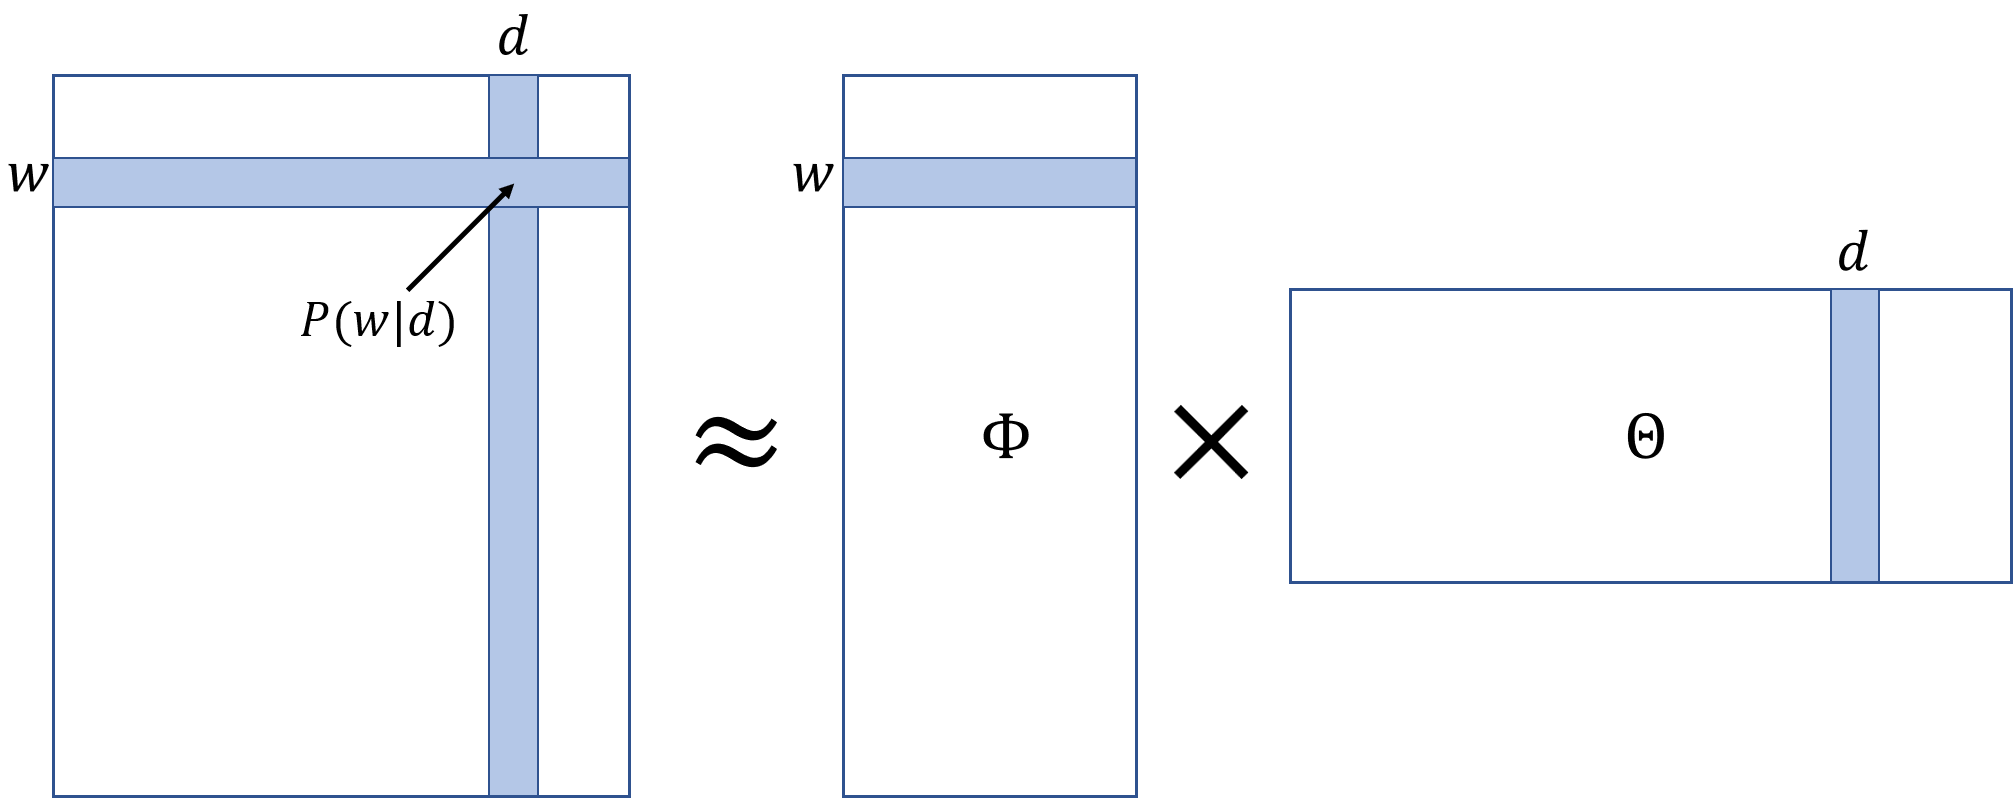
\includegraphics[scale=0.5]{svd.png}
    \caption{Стохастическое разложение матриц}
    \label{fig:svd}
\end{figure}